\chapter{Implementation and Methods} % Main chapter title

\label{Chapter3} % For referencing the chapter elsewhere, use \ref{Chapter1} 

\section{What to do with this research}
In this section we will discuss the methods that have been compiled for the literature review discussed in Chapter \ref{Chapter2} and how algorithms have been constructed. We will also detail the testing procedure for the new algorithms and how to assess the validity and reliability of these methods. In the final section will discuss the initial assumptions. 

\section{Algorithms and Design}
We will explore in detail the algorithms that will be implemented for the PDDL4J library and how the research brought us to the conclusion that these algorithms are more efficient than the existing ones. The search algorithm and heuristic have been taken from previous work in the classical planning field and applied to the PDDL4J planner.

As the PDDL4J library is written in Java, the best way to implement the new algorithms is to use the existing parser and lexer for the library and then remove all existing code for the A* algorithm and implement the new GBFS and EHC at the top level. As creating the parser and lexer would be a lot of work, we felt this was the better option as the existing code was efficient at parsing the domain and problem files. 

The two search algorithms were available in pseudo-code which made the implementation a lot easier. The enforced hill climbing has been used multiple times so information regarding it was widely available\cite{HeuristicDomain}. The two new algorithms will be broken down into the following sub-sections and evaluated. 
\subsection{Greedy Best First Search with Enforced Hill Climbing}
From the research conducted on search algorithms, we have made the decision to implement Enforced Hill Climbing (EHC) which was used in the Fast Forward planner \cite{FFPlanner} but instead of using A* or a modified version of it, we have decided to use a generic Greedy Best First Search algorithm\cite{AModernApproach}. The main reason for implementing EHC is due to its success at previous IPC competitions as well as being able to be implemented alongside another search algorithm like GBFS. We felt that it would improve the PDDL4J library in terms of speed, memory and solving problems.
As GBFS expands the node that appears closest to the goal and uses the function $f(n) = h(n)$. This means that it only uses the heuristic to guide the search. So if we incorporate GBFS as a back-up algorithm for EHC with the Fast Forward heuristic, this will make a faster/more memory efficient planner than A* with the Fast Forward heuristic which is what is used within the library at present. 
From the work carried out by Blai Bonet and Hector Geffner, they proposed changing an old planner HSP \cite{HeuristicNewResults} from a hill climbing algorithm to a Best First Search algorithm, and the results showed that there was a dramatic increase in the number of solved problems compared to just using EHC \cite{PlanningHeuristic}. One reason we want to combine these two algorithms is that the EHC algorithm is not complete and it has a problem with potentially getting stuck in infinite loops so we want to include GBFS as well as a relaxed heuristic like Fast Forward. 
Another main driving point why we think that A* can be beaten in terms of speed/memory consumption is that, in previous research, it states that A* is slower than other searching algorithms due to the computation of $h(s)$ for every new state, which is computationally expensive\cite{HeuristicNewResults}, therefore, we want to avoid this computation if possible. The decision was then made to incorporate the EHC and GBFS together to create potentially a fast, memory conscious planner that would rival A*.  
\\
We have already introduced the EHC in Chapter \ref{Chapter2} as well as talked a little about GBFS but now we will describe how these two algorithms will work in depth and how they can complement each other. 
The use of a GBFS means that we will greedily expand the first successor that is found with a better heuristic value than its parent. But the algorithm will keep the parent stored so that the remaining children can be evaluated later. This, in turn, means that when we generate a successor state, two things can happen: 
\begin{itemize}
\item if the heuristic value of a successor is better than the parent, the parent is placed behind the successor in the search queue; or
\item if the heuristic value is not better than the parent, we use the value of the successor to place it in a priority queue and we continue the search.  
\end{itemize}
In algorithm 4, we can see the pseudo-code for the GBFS algorithm. The aim is to perform heuristic evaluations that will be low as we envisage fewer successors.\cite{GreedyOnline} 
\begin{algorithm}[H]
\caption{Greedy Best First Search}
\begin{algorithmic}
\State state = initialState 
\State h = initialHeuristic
\While {searchQueue \textbf{is not } empty}
\State currentQuery = pop item from front of searchQueue
\State currentState = state from currentQuery
\State currentHeuristic = heuristic from currentQueue
\State applicableActions = array of actions applicable in currentState
\ForAll{index $\in$ applicableActions $\geq$ counter}
\State currentAction = applicableActions
\State successorState = currentState.apply(currentAction)
\If {successorState = goal}
\State return(plan)
\EndIf
\State successorHeuristic = heuristicValue(successorState)
\If {successorHeuristic < currentHeuristic}
\State inset(currentState, currentHeuristic) 
\State insert(successorState, successorHeuristic)
\Else { insert(successorState, successorHeuristic}
\EndIf
\EndFor
\EndWhile
\end{algorithmic}
\end{algorithm}

An advantage in GBFS is that it can be a forward or backward search algorithm. In this case we will use it as a forward search and it falls into the category \textit{state space algorithm}, i.e. it looks through the space of possible states instead of looking for partial plans. With the implementation of these two new algorithms I purposed that the use of the Fast Forward heuristic that has been built within the PDDL4J library will be able to solve more problems than A* with Fast Forward and in faster times, as well as use less memory.

\subsection{$H^m$ Heuristic} 
Here we will define the $H^m$ heuristic that was developed by Patrik Haslum and Hector Geffner\cite{AdmissibleHeuristic}. The $H^m$ heuristic is a domain-independent admissible heuristic which can be used to create optimal plans. This heuristic is part of the family of heuristics discussed in \ref{Chapter2} where we change a small section of the Max heuristic to create the $H^m$ heuristic. 
The new heuristic is based on computing admissible estimates of the costs of achieving sets of atoms from the initial state\cite{AdmissibleHeuristic}. This means that when we have a set of these atoms of size 1, it is basically equivalent to the Max heuristic.
\begin{equation}
\begin{aligned}
& h^m(g,s) = 0 \textbf{ if } g \subseteq s\\
& h^m(g,s) = \infty \textbf{ if } g \not\subseteq s
\end{aligned}
\end{equation}
The above equation is the beginning of the algorithm. It is stating that if the goal exists within the state $s$ then it is 0, and if it is not within the state then the node is unexplored so its set to infinity.
\begin{equation}
\begin{aligned}
& \textbf{if } |g| \leq k\\
& min_a (1 + \bigtriangleup^*(s, \lambda^{-1}(g,a)) | a\ relevant\ for\ g)\\
& \textbf{otherwise}\\
& max_{g'}(\bigtriangleup_k(s,g') | g'\subseteq g\ and\ |g'| = k
\end{aligned}
\end{equation} 
This was taken from \cite{PlanningBook} and it means that when $g$ has at most $k$ propositions, we take the exact value $\bigtriangleup^*$ but if that is not possible then we approximate the distance $\bigtriangleup_k$ to $g$. 
We then can break down this algorithm to give it more meaning – looking through \cite{PlanningBook} we see that $\lambda^{-1}(g,a)$ can be defined as:
\begin{equation}
\lambda^{-1}(g,a) = (g - effects^+(a) \cup precond(a)
\end{equation}  
Then further looking redefines $a$ to be relevant for $g$	 as:
\begin{equation} 
g \cap effects^+(a) \neq 0 \wedge g \cap effects^- = 0
\end{equation}
In\cite{PlanningBook}\cite{AdmissibleHeuristic} they both have recommended that the value of $k$ is kept at 2 because, as problems get harder with more objects, it is computationally expensive to generate subsets. The complexity of the heuristic makes the computation a polynomial $N^k$ where $N$ is the number of atoms. 
\section{How to Evaluate}
Based on a research paper by Carlos Linares Lopez, the new algorithms will be evaluated using the techniques discussed in \cite{Evaluation}. We will use all of the evaluation techniques as this will give a better idea of how effective the new algorithms are for the PDDL4J planner. 
The evaluation criteria is broken down into the following 4 categories:
\begin{itemize}
\item Objectivity – We want to have the same setting for all tests
\begin{itemize}
\item Representation Language – Keep the same order for each domain and problem as this can affect the outcome. Also the language used i.e. PDDL 
\item Evaluation Metric – Use one metric like time, plan size etc or if using multiple, keep it consistent throughout
\item Validation – Use a reliable system to validate the plans. It will ensure that the solution plans are logically sound 
\end{itemize}
\item Exhaustiveness – Use problems of a different nature, i.e. STRIPS and ADL, as well as multiple problem files within a domain which keeps the same problem structure but changes initial states and goal states
\item Comparability – Using well studied algorithms as a baseline for the new algorithms
\item Reproducibility – The test environment must be detailed so it can be replicated  
\end{itemize}
\subsection{How We Will Achieve This}
Within the domain of classical planning, the IPC competition has a number of domains and problems that are used each year to test the planners. So for the testing procedure, we have taken a number of domains and problems from each year of the IPC competition to make an extensive set of testing domains which will give a fair analysis of the new algorithms and methods. The tests will be run on a Linux server that has 24 CPUs, each Intel(R) Xeon(R) 2.30GHZ, as well as having 264.13GB of memory, which is more than capable of running the new algorithms. Each problem will be allowed 10 minutes to find a solution but if no solution is found within the time limit then the planner will skip and go on to the next problem. 

We will be using a piece of software called GNU parallel\cite{GNU} so the problems can be run sequentially to save time, however, the issue is that the threads that have been created to execute problems will be sharing resources so we need to try to limit the resources so that each thread has a specific amount. Below shows an example of one way we can use GNU parallel to test the program. The $seq$ allows us to start with the first problem and finish at the final problem (in this case 20). The $-j 6$ tells the server that we want 6 processes to be created and to run sequentially. The next part is allocating memory to each of the processes. We are opting for 8048 megabytes as we think this is a fair amount of memory for the planner. 
\begin{verbatim}
seq -w 20 | parallel -k -j6 java 
-javaagent:build/libs/pddl4j-3.1.0.
jar -server -Xms8048m -Xmx8048m 
fr.uga.pddl4j.planners.hsp.HSP -o 
pddl/benchmarks_STRIPS/ipc1/gripper/domain.pddl -f
pddl/benchmarks_STRIPS/ipc1/gripper/p{}.pddl 
-i 8 '>>' AstarGripper.txt
\end{verbatim}
There will be a variety of STRIPS and ADL problems within the tested domains. Each of the domains will have a range of problems from small to medium and hard. All of the actions within each domain will be listed in the same order, as well as the problem files. The domains that we will be testing are in the table below: the left column shows the domain name, the middle column shows the number of problems in each domain and the right column shows which IPC competition they are from. 
\begin{center}
  \begin{tabular}{ | l | c | r |}
    \hline
    \textbf{Domain} & \textbf{Number of Problems} & \textbf{IPC} \\ \hline
    Gripper & 20 & IPC1 \\ \hline
    Logistics & 30 & IPC1 \\ \hline
    Movie & 30 & IPC1 \\ \hline
    Mprime & 30 & IPC1 \\ \hline
    Mystery & 30 & IPC1 \\ \hline
    Blocksworld & 35 & IPC2 \\ \hline
    Elevator & 100 & IPC2 \\ \hline
    Freecell & 60 & IPC2 \\ \hline
    Schedule & 100 & IPC2 \\ \hline
    Depots & 22 & IPC3 \\ \hline
    Driverlog & 20 & IPC3 \\ \hline
    Rover & 20 & IPC3 \\ \hline
    Satellite & 20 & IPC3 \\ \hline
    Zenotravel & 20 & IPC3 \\ \hline
    Airport & 50 & IPC4 \\ \hline
    Optical Telegraph & 14 & IPC4 \\ \hline
    Philosophers & 29 & IPC4 \\ \hline
    Pipesworld & 50 & IPC4 \\ \hline
    Psr & 50 & IPC4 \\ \hline
    Openstacks & 30 & IPC5 \\ \hline
    Pathways & 30 & IPC5 \\ \hline
    Storage & 30 & IPC5 \\ \hline
    Tpp & 30 & IPC5 \\ \hline
    Truck & 30 & IPC5 \\ \hline
    Pegsol & 30 & IPC6 \\ \hline
    Sokoban & 30 & IPC6 \\ \hline
    Transport & 30 & IPC6 \\ \hline
    Barman & 20 & IPC7 \\ \hline
    Nomystery & 20 & IPC7 \\ \hline
    Parking & 20 & IPC7 \\ \hline
    Childsnack & 20 & IPC8 \\ \hline
    Hiking & 20 & IPC8 \\ \hline
    Thoughtful & 20 & IPC8 \\
    \hline
  \end{tabular}
\end{center}
The main test is the search algorithms, and they will be tested with the same procedure and the results will be compared in three areas:
\begin{itemize}
\item Time – How fast the planner can find a valid plan
\item Memory – What is the consumption of memory used to compute a valid plan
\item Plan size – What are the number of actions been completed to solve a problem 
\end{itemize}
Both search algorithms will use the heuristic Fast Forward and will be tested in the same environment. 
The new heuristic will be tested against three other heuristics: Max, Sum and Fast Forward. They will be tested using the same search algorithm (A*) and then compared in the same format as above but with one extra measurement, i.e. plan quality. This is where we look at each plan individually and assess when actions were executed to see if the admissibility of certain heuristics is true or false. Also, we will see how not admissible heuristics complete a plan and the steps they take compared to an admissible heuristic.
\subsection{Validity}
Validity is defined as \textit{"the quality of being logically or factually sound; soundness or cogency".} \cite{ValidityDef} In the context of this thesis, we will be using a plan-checking software that was used for the IPC 2002 competition\cite{ICAPS2002} which incorporates STRIPS and ADL (the use of which was decided in Chapter \ref{Chapter2} of this thesis). The plan-checking software was built for the competition by Stephen Cresswell and it works by generating parse trees for PDDL 2.1 syntax. It uses a range of different coding languages and functions to check if a plan is logically sound.
\textit{"A state-space planner provides a plan as a sequence of actions"}\cite{PlanningBook}. This is the goal for the new algorithms, i.e. to provide a sequence of actions that are logically sound, for example:
\\
\begin{figure}[!htb]
    \centering
    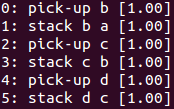
\includegraphics[scale=1]{SoundPlan.png}
    \caption{Example of a sound plan from Blocksworld}
    \label{fig:SoundPlan}
\end{figure}
\\
We can see from Figure \ref{fig:SoundPlan} above that there are no instances where the plan is incorrect. So at each step in the plan, the actions can be executed. An example of a non logically sound plan would be if, at step 2, the planner executed the action \textit{pick-up b}; this would not be possible unless the planner unstacked \textit{b} and \textit{a} first. 
\\
For validity we used a system called VAL which is a plan validator \cite{VAL}. It takes in a domain file, a problem file, a plan file, and tests to see if the plan is feasible given the set of actions in the domain and the problem.  
\section{Initial Assumptions}
The initial assumptions for the new search algorithm (GBFS with EHC using the Fast Forward heuristic) are that it will be able to provide a plan in a faster time and with less memory consumption than A* as well as being able to solve more problems from within the total amount. 
The new heuristic ($H^m$) will provide a critical path from starting node $s_0$ to a goal node $s_n$. In other words, the heuristic will sacrifice time and memory consumption but provide the optimal path. In comparison to other admissible heuristics where the plan length will be the same, we assume that the $H^m$ heuristic will complete different actions than other admissible heuristics in order to achieve a goal. 